\chapter[Introduction]{Introduction} 
\label{chap:Intro} \index{Introduction}

\newepigraph{In the strict formulation of the law of causality - if we know the present, we can calculate the future - it is not the conclusion that is wrong, but the premise.}
{Werner Heisenberg}

A significant part of scientific applications demand the forecasting of natural, social and economical processes and there is an extensive literature on forecasting methods and models. Such methods are also preceded by many  processes as instrumentation, measurement, storing, aggregation, etc. However, a great recurrent problem is how to deal with the uncertainty generated or captured in each step of this task, and measure how it spreads. \cite{Makridakis2009} stated that ``Statistical models underestimate uncertainty, sometimes catastrophically'', by assuming, for example, that events are independent, forecasting errors are tractable, the variance of forecasting errors is finite, known and constant. 

\index{Ontological uncertainty}\index{Intrinsic uncertainty}\index{Irreducible uncertainty}

In these natural and social processes the uncertainty can be intrinsic or extrinsic and is classified, by \cite{Georgescu2014}, in two categories: the epistemic uncertainty and the ontological uncertainty. The ontological uncertainty represents the intrinsic and irreducible uncertainty of a process defined basically as the non-deterministic behavior -- randomness and stochasticity -- that usually is modeled by the probability theory. 

\index{Epistemic uncertainty}\index{Extrinsic uncertainty}\index{Reducible uncertainty}

Contrarily, the epistemic uncertainty represents the extrinsic and reducible sources of uncertainty on a process like vagueness, lack of information and imprecision due to measurement errors, sensor calibration, rounding and limitations of numerical precision, among others. Another possibility is the conversion of continuous processes to discrete processes. This conversion is not lossless and some uncertainty is imputed on converted data. The epistemic uncertainty can be modeled by the fuzzy theory. 

This is the case of data preprocessing tasks, for example. Very often time series datasets need to be aggregated by some time resolution (daily, hourly, etc) and this aggregation also introduces the epistemic uncertainty on data. A good example are the financial time series that summarize all transactions of a whole day in four numbers: opening, minimum, maximum and closing prices. This method is an attempt to represent the volatility (e. g. the uncertainty) of the price value inside a certain time window and is also a tool for detecting patterns on data, the Candlestick Graph techniques, as shown in Figure \ref{fig:candlestick}. Sometimes the aggregation is even more aggressive and all the values are summarized into one, the average or median value, hiding all information about the volatility. When this data is used as input for fitting a forecasting model the extrinsic uncertainty is introduced.

\begin{figure}
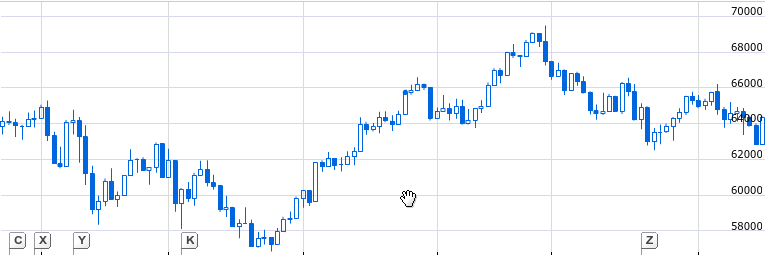
\includegraphics[width=\textwidth,height=2in]{figures/candlestick.png}
\caption[Candlestick chart for IBOVESPA]%
{Candlestick chart for IBOVESPA. Source: Google Finance\protect\footnotemark}
\label{fig:candlestick}
\end{figure}

\footnotetext{\url{https://www.google.com/financeq=INDEXBVMF\%3AIBOV&ei=zHz2WOmMKODrep_bgbAI}. Access in 18/04/2017}

The forecasting methods propagate the input uncertainties on their outputs and compromise the reliability of the forecast. Despite these points, the majority of forecasting methods are concerned with one step ahead point forecasting without output uncertainty measures. When the many steps ahead forecasting is considered, the uncertainty grows yet more and affects the accuracy and reliability of models. This effect becomes even worst  as the forecasting horizon becomes wider.

This fact led to the development of methods for Probabilistic Forecasting \cite{Gneiting2014b} and  Interval Forecasting \cite{Chatfield1993},  to deal with forecasting uncertainty by estimating distributions of possible values instead of a unique point forecast. However, traditional methods of probabilistic forecasting require the use of parametric models with distribution assumptions, as in Bayesian Inference, or costly estimation techniques and Monte-Carlo simulations. Probabilistic forecasting has been used in areas such as weather forecasting (\cite{Fraley2011} and \cite{Leutbecher2008}) eletric load forecasting (\cite{Hong2016}, \cite{Hong2016a} and \cite{Liu2015}), wind power generation prediction (\cite{Pinson2006} and  \cite{Netto2016}) and hydrological forecasting (\cite{Laio2007}).

Side by side with the uncertainty representation in time series forecasts, some other factors became prevailing in the evaluation of predictive methods, such as Big Data scalability and model explainability. The Big Data phenomenon emerged in the late 2000s decade \cite{Lynch2008} calling attention to new demands on data analysis brought by the growth of data volume, dimensionality and variety. This revolution was possible due to the advances on the technologies of data capturing and storage, as well as its commoditizing, allowing the distributed management of amounts of data never seen before. 

But traditional forecasting methods, and even some newer ones, were not designed to deal with such high volume of data. The most critical issues were the high dimensionality  (dozens of hundreds of attributes) and volume (hundreds of millions or billions of samples) \cite{Qiu2016}. Such data volume cannot be grounded on a single machine memory and demands a distributed architecture of storage and processing. New technologies emerged to tackle these issues, for instance the Map Reduce based frameworks \cite{Dean2008}, a divide-and-conquer approach which is the basis of Hadoop clusters \cite{White2012}, where the processing units also act as storage units of the data subsets using commodity and cheap hardware assets.

The Big Data issues do not stop on data volume and, indeed, the velocity and variability of the data must be seriously considered when developing forecasting models. Many sources of data have non-stationary behaviors, meaning that their statistical properties may change along the time. Some models are time-variant, they are specially designed to be self-adaptable and evolve as the data change. But the majority of the  conventional methods are time-invariant and need to be retrained periodically depending on the variability of the data, what can be problematic given the computational cost of the training and adapting procedures. Yet more critical is the data with Concept Drifts \citep{Gama2014}, which have high volume with high velocity and need to be adaptable to new behaviors in feasible time. 

Another traditionally neglected aspect of the forecasting methods also started to gain more attention in recent years: the explainability. With the expansion of the machine learning methods enabled to tackle Big Data, another issues came up to the light: black-box methods started to find legal barriers or adoption resistance due to its lack of transparency and auditability \citep{Leslie2019, ECAIHLEG2019}. Diversely, the white-box methods can help in the knowledge extraction and simplification of complex temporal patterns, besides being easily auditable.

%If all these concerns (uncertainty representation,  scalability, low computational cost, explainability and self-adaptability) were taken in account, it becomes pretty hard to find a fitting method. But several of these issues
%the development of new soft-computing methods
The exposed scenario favored the rising of the Fuzzy Time Series (FTS) methods \cite{song1993fuzzy}, which have been drawing more  attention and relevance in recent years due to many studies reporting its good accuracy compared with other models \cite{Singh2008}. Fuzzy Time Series are soft-computing methods that produce data-driven, non-parametric, simple, computationally cheap and readable models for time series analysis and forecasting. FTS methods are also an approach to deal with  the  epistemic uncertainty, as on the time-aggregation case of the financial time series. The fuzzyfication of data gives a more flexible representation to the individual measures, embracing the range of possible value fluctuations not covered by the single values. 

Despite the great improvements published in the FTS literature in the recent years, there are still some notable lacks. Interval and probabilistic forecasting, specially for many steps ahead, are not properly explored, besides the absence of scalable methods to tackle big multivariate time series. There is, indeed, a plethora of soft-computing forecasting methods. But very few of them are flexible enough to incorporate scalable point, interval, probabilistic and multivariate forecasting, with one to many steps ahead, for univariate and multivariate time series. This research opportunity is exploited in this work by the proposition of new FTS methods and their subsequent applications on several case studies, including financial, environmental and energy time series. 

\section{Objectives} \index{Objectives} 

The main goal of this thesis is to develop a scalable probabilistic forecasting approach based on the Fuzzy Time Series methods, providing a flexible computational framework for applications with uncertainties. Specific goals are divided in:

\begin{itemize}
\item Identify the strengths and weaknesses of the main FTS approaches presented in literature;
\item Identify extension opportunities on known probabilistic forecasting methods;
\item Introduce the Probabilistic Weighted Fuzzy Time Series, a new method family that exploits uncertainties on datasets to capture time series patterns and translate them into the rule-based knowledge system (the Probabilistic Weighted Fuzzy Logical Relationship Groups);
\item Improve PWFTS scalability in order to enable it to deal with big time series by proposing a distributed processing design with the Map/Reduce paradigm; 
\item Extend the PWFTS method to enable multivariate time series using Fuzzy Information Granules.
\end{itemize}

\section{Work structure} \index{Work structure}

This thesis is organized as follows:

\begin{itemize}
\item \textbf{Chapter \ref{chap:review_fts} - \nameref{chap:review_fts} } presents a contextual background on Fuzzy Time Series methods and discusses the most relevant methods in literature;

\item \textbf{Chapter \ref{chap:review_probforecasting} - \nameref{chap:review_probforecasting} } introduces the probabilistic forecasting concepts and main techniques, reviewing the surrounding literature. In Section \ref{sec:ifts} the Interval Fuzzy Time Series method is proposed for binding the fuzzy uncertainty on forecasts, and in Section \ref{sec:ensemblefts} the EnsembleFTS method is proposed to probabilistic forecasting;

\item \textbf{Chapter \ref{chap:pwfts} - \nameref{chap:pwfts}} introduces the Probabilistic Fuzzy Time Series method for generating the Probabilistic Weighted Fuzzy Temporal Pattern rules and a method to generate one step ahead probabilistic forecasts; in Section \ref{sec:pwfts_interval} the previous method is extended to create prediction intervals and in Section \ref{sec:pwfts_point} a simple heuristic to produce point forecasts is presented . Section \ref{sec:pwfts_extensions} presents extensions for many steps ahead forecasting and high-order models. The characteristics and parameters of the methods are discussed in Section \ref{sec:pwfts_experiments};

\item \textbf{Chapter \ref{chap:scalability} - \nameref{chap:scalability}} proposes a distributed approach for PWFTS, based on Map/Reduce paradigm and computational clusters, enabling it to deal with big time series. In Section \ref{sec:hyperparameter} the Distributed Evolutionary Hyperparameter Optimization (DEHO) is proposed, employing evolutionary algorithms with the distributed processing to improve the performance.

\item \textbf{Chapter \ref{chap:multivariate} - \nameref{chap:multivariate}} proposes an extension for multivariate time series using Fuzzy Information Granules (FIG) and an incremental universe of discourse partitioner. With this extension PWFTS can be used for multivariate forecasting in a Multiple Input/Multiple Output (MIMO) design or monovariate forecasting in a Multiple Input/Single Output(MISO) design.

%\item \textbf{Chapter \ref{chap:results} - \nameref{chap:results}} an empirical analysis is employed to validate the proposed method, using open datasets and standard measures, and to compare its performance with others well-known literature methods.

\item \textbf{Chapter \ref{chap:conclusions} - \nameref{chap:conclusions}} the findings are summarized and overall conclusions are given, as well as the contributions, known limitations and future investigations. 
\end{itemize}

\section{Main contributions} \index{Contributions}

This research presents contributions to the Forecasting and Fuzzy Time Series research fields, whose the most important are summarized below:

\begin{itemize}
    \item Proposal of new High Order Fuzzy Time Series (HOFTS) and the Weighted HOFTS, methods that aggregate the major FTS features present in the literature and play the role of the consensus of the FTS methods;
    \item Proposal of the first FTS methods to perform interval forecasting, the Interval Fuzzy Time Series ($\ifts$) and the Weighted $\ifts$;
    \item Proposal of the first FTS method to perform probabilistic forecasting, the Ensemble FTS;
    \item Proposal of the Probabilistic Weighted Fuzzy Time Series - PWFTS, a new non-parametric, data driven and highly accurate forecasting method, the first FTS method in the literature that integrates point, interval and probabilistic forecasting in the same model, for one to many steps ahead;
    \item A new representation method for fuzzy temporal rules, with weights on the precedent and the consequent of the rules, reflecting its \textit{a priori} and \textit{a posteriori} empirical probabilities and aiding with model explainability;
    \item New defuzzyfication methods capable to produce probability distributions, prediction intervals and point forecasts;
    \item Proposal of distributed training and forecasting methods that allow PWFTS to work with big time series using Map/Reduce framework;
    \item Proposal of the Distributed Evolutionary Hyperparameter Optimization (DEHO) method for PWFTS;
    \item Proposal of the Multivariate Fuzzy Time Series and (MVFTS) the Weighted MVFTS, simple multivariate fuzzy time series;
    \item Proposal of the $\FIG$-FTS, a wrapper method that allow PWFTS to work with multivariate time series;
    \item Proposal of the pyFTS library \cite{pyFTS}\footnote{\url{http://pyfts.github.io/pyFTS/}} for Python programming language, an open and free framework to facilitate the development of new models and help on research reproducibility;  
    \item The application of the proposed methods in the forecasting of renewable energy and environmental processes;
\end{itemize}


